\documentclass[aspectratio=169,notheorems,10pt]{beamer}

\usepackage{algorithm}
\usepackage[noend]{algpseudocode}
\usepackage{amsfonts}
\usepackage{amssymb}
\usepackage{amsthm}
\usepackage{bm}
\usepackage{booktabs}
\usepackage{hyperref}
\usepackage[scr=boondox]{mathalpha}
\usepackage{mathtools}
\usepackage{mleftright}
\usepackage[round]{natbib}
\usepackage{parskip}
\usepackage{physics}
\usepackage{tabularx}
\usepackage{tikz}
\usepackage{xcolor}
\usepackage{xparse}

\addtobeamertemplate{itemize/enumerate body begin}{}{
	\setlength{\itemsep}{2pt}
	\setlength{\parskip}{2pt}
	\setlength{\parsep}{2pt}
}
\addtobeamertemplate{itemize/enumerate subbody begin}{}{
	\setlength{\itemsep}{2pt}
	\setlength{\parskip}{2pt}
	\setlength{\parsep}{2pt}
}

\useinnertheme{circles}
\useoutertheme[subsection=false]{miniframes}
\setbeamertemplate{navigation symbols}{}

\usetikzlibrary{positioning, arrows.meta}

\algrenewcomment[1]{{$\triangleright$\text{\ }\textit{#1}}}
\setcounter{MaxMatrixCols}{30}

\theoremstyle{definition}
\newtheorem{definition}{Definition}
\newtheorem{notation}{Notation}
\newtheorem{theorem}{Theorem}
\newtheorem{proposition}{Proposition}
\newtheorem{claim}{Claim}
\newtheorem{remark}{Remark}

\makeatletter
\def\thm@space@setup{\thm@preskip=\parskip \thm@postskip=0pt}
\makeatother

\let\oldhref\href
\renewcommand{\href}[2]{\oldhref{#1}{\textbf{#2}}}

\DeclareMathOperator*{\argmax}{arg\,max}
\DeclareMathOperator*{\argmin}{arg\,min}
\newcommand{\E}{\mathbb{E}}
\newcommand{\N}{\mathbb{N}}
\newcommand{\R}{\mathbb{R}}
\newcommand{\Z}{\mathbb{Z}}

\title{SUTD404: Denoising Language Models\\for Room-to-Address Lookup}
\author{
	G. Lim,
	E. Ang,
	M. Shaswat,
	M. Ramaswamy
}
\date{April 2026}

\begin{document}

\maketitle

\section{Introduction}
\begin{frame}
\begin{itemize}
	\item SUTD has over 200 rooms across 5 buildings.
	\item Rooms are often communicated by name.
	\item Room-to-address lookup can be a hassle.
\end{itemize}
\end{frame}

\begin{frame}
\begin{itemize}
	\item Resources for this task remain limited.
	\item Physical signs often require one to walk around.
	\item Digital resources like the SUTD Assistive Maps (SAM) Telegram bot often fail on noisy input (e.g. strings with typos).
\end{itemize}
\end{frame}

\begin{frame}
\begin{itemize}
	\item We introduce SUTD404 to address this gap.
	\item Visit \href{https://github.com/gregorylimeurhen/sutd404}{github.com/gregorylimeurhen/sutd404} for our code repository.
	\item Visit \href{https://sutd404.vercel.app}{sutd404.vercel.app} for our web application.
\end{itemize}
\end{frame}

\section{Methodology}

\begin{frame}[fragile]
\begin{definition}[Keyboard]
$${\setlength{\arraycolsep}{2pt}
	K
	=
	\begin{bmatrix}
		\texttt{`} & & \texttt{1} & & \texttt{2} & & \texttt{3} & & \texttt{4} & & \texttt{5} & & \texttt{6} & & \texttt{7} & & \texttt{8} & & \texttt{9} & & \texttt{0} & & \texttt{-} & & \texttt{=}
		\\
		\texttt{q} & & \texttt{w} & & \texttt{e} & & \texttt{r} & & \texttt{t} & & \texttt{y} & & \texttt{u} & & \texttt{i} & & \texttt{o} & & \texttt{p} & & \texttt{[} & & \texttt{]} & & \verb|\|
		\\
		& & \texttt{a} & & \texttt{s} & & \texttt{d} & & \texttt{f} & & \texttt{g} & & \texttt{h} & & \texttt{j} & & \texttt{k} & & \texttt{l} & & \texttt{;} & & \texttt{'} & &
		\\
		& & & \texttt{z} & & \texttt{x} & & \texttt{c} & & \texttt{v} & & \texttt{b} & & \texttt{n} & & \texttt{m} & & \texttt{,} & & \texttt{.} & & \texttt{/} & & & &
		\\
		& & & & & & & & & & \texttt{\textvisiblespace} & \texttt{\textvisiblespace} & \texttt{\textvisiblespace} & \texttt{\textvisiblespace} & \texttt{\textvisiblespace} & & & & & & & & & &
	\end{bmatrix}
}$$
\end{definition}
\begin{itemize}
	\item We define a 60\% ANSI QWERTY en-US keyboard layout.
\end{itemize}
\end{frame}

\begin{frame}
\begin{figure}[H]
	\centering
	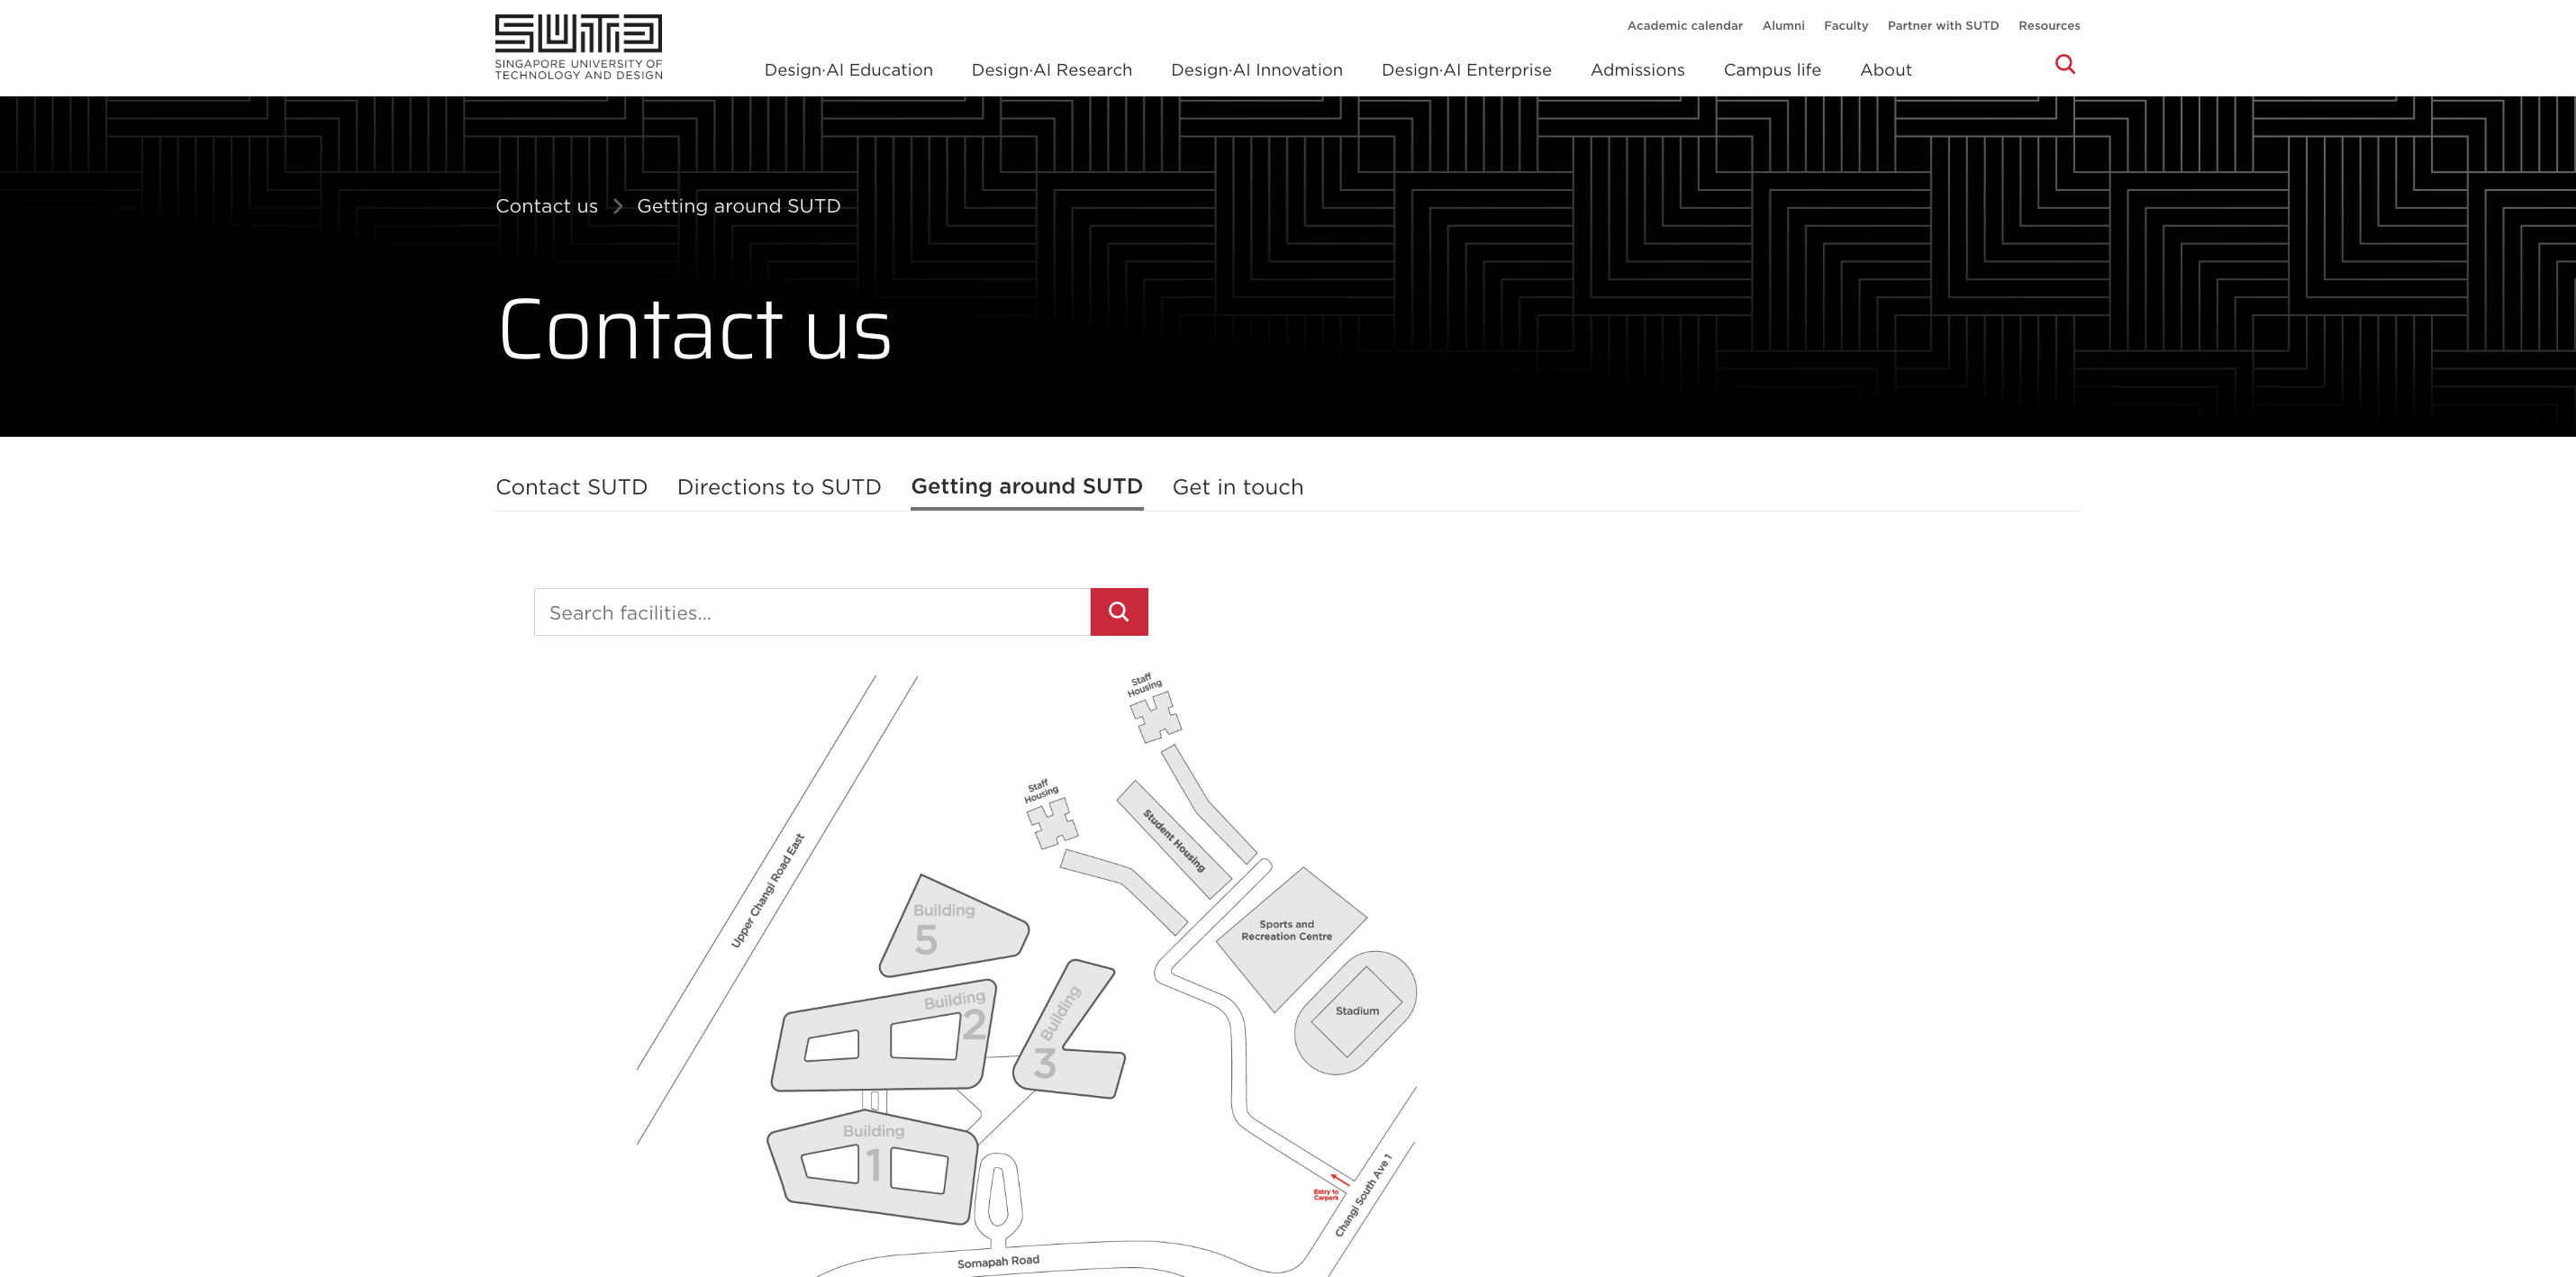
\includegraphics[width=0.5\linewidth]{contact.png}
	\caption{Official SUTD contact pages.}
\end{figure}
\begin{itemize}
	\item We obtain a room set $R$ by politely scraping official SUTD contact pages.
	\item We queried the facility search function by enumerating buildings and floors.
\end{itemize}
\end{frame}

\begin{frame}
Let $V$ be a vocabulary,
and $R\subseteq V^{*}$ be a room set,
and $\prec$ be a total order on $R$,
and $N\in\N_{\geq 1}$ be a result count,
and $\prec_{N}$ be a total order on $R_{\prec}^{N}$,
and $A\subseteq V^{*}$ be an address set,
and $B\subseteq V$ be a boundary set,
and $C\in\N$ be a corruption count,
and $\alpha\in\R_{[0,1]}$ be a transposition rate,
and $\beta\in\R_{[0,1]}$ be a substitution rate,
and $\bm{\pi}=(\pi_\mathrm{train},\pi_\mathrm{val},\pi_\mathrm{test})\in\Delta_{C}^{2}$ be a training-validation-testing split,
and $I:V\rightharpoonup\Z^{2}$ be a keyboard-position map.
\end{frame}

\begin{frame}
\begin{algorithm}[H]
	\caption{$\textsc{Corrupt}(\bm{x})$}
	\begin{algorithmic}
		\Require $\bm{x}\in V^{*}$
		\State ${
			(T_{L},T_{M},T_{R})
			\gets
			(V^{*}B\cup\{()\},(V\setminus B)^{+},BV^{*}\cup\{()\})
		}$
		\State ${
			T
			\gets
			\{
				\bm{u}\bm{w}b\bm{v}\bm{z}
				\mid
				\bm{u}\in T_{L},\,
				\bm{v},\bm{w}\in T_{M},\,
				\bm{z}\in T_{R},\,
				b\in B,\,
				\bm{x}=\bm{u}\bm{v}b\bm{w}\bm{z}
			\}
			\setminus
			\{\bm{x}\}
		}$
		\If{$T\neq\varnothing$}
			${\bm{x}\sim\alpha\,\mathcal{U}(T)+(1-\alpha)\,\delta(\bm{x})}$
		\EndIf
		\For{$i\in[1..\abs{\bm{x}}]$}
			\State ${
				S
				\gets
				\{
					k\in K
					\setminus
					\{x_{i}\}
					\mid
					I(k)-I(x_{i})
					\in
					[-1..1]
					\times
					[-2..2]
				\}
			}$
			\If{$S\neq\varnothing$}
				${x_{i}\sim\beta\,\mathcal{U}(S)+(1-\beta)\,\delta(x_{i})}$
			\EndIf
		\EndFor
		\State \Return $\bm{x}$
	\end{algorithmic}
\end{algorithm}
\begin{itemize}
	\item We generated corrupted strings and split corrupted-uncorrupted room pairs into training, validation, and testing datasets:
	\begin{itemize}
		\item Our corruption algorithm transposes spans and substituting characters.
		\item We set $C=50$, and $\alpha=0.5$, and $\beta=0.05$, and $\bm{\pi}=(0.8,0.1,0.1)$ for tractable and plausible-looking typos.
		\item We stratify the split by room to make the datasets comparable across rooms.
	\end{itemize}
\end{itemize}
\end{frame}

\begin{frame}
\begin{figure}
	\centering
	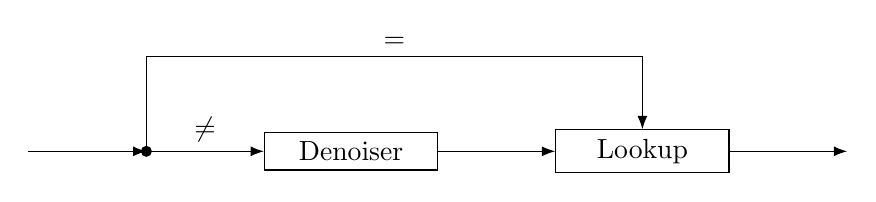
\begin{tikzpicture}[>=Latex]
		\def\L{1.5}
		\def\W{2.2}
		\def\H{1.2}

		\coordinate (input) at (-\L,0);
		\coordinate (split) at (0,0);

		\node[draw, minimum width=\W cm] (denoiser)
			at ({\L + \W/2},0) {Denoiser};

		\node[draw, minimum width=\W cm] (lookup)
			at ({2*\L + 3*\W/2},0) {Lookup};

		\coordinate (output) at ({3*\L + 2*\W},0);
		\coordinate (above-split) at (0,\H);
		\coordinate (above-lookup) at ({2*\L + 3*\W/2},\H);

		\draw[->] (input) -- (split);
		\draw[->] (split) -- node[above] {$\neq$} (denoiser.west);
		\draw[->] (denoiser.east) -- (lookup.west);
		\draw[->] (lookup.east) -- (output);
		\draw[->] (split) -- (above-split)
			-- node[above] {$=$} (above-lookup)
			-- (lookup.north);

		\fill (split) circle (2pt);
	\end{tikzpicture}
	\caption{Inference algorithm.}
\end{figure}
\end{frame}

\begin{frame}
\begin{definition}[Denoiser]
Let $f:V^{*}\times R\to\R$ be a scorer.
\begin{align*}
	\mathscr{D}_{f}
	&:
	V^{*}\to R
	\\
	\mathscr{D}_{f}(x)
	&=
	\min_{\prec}
	\argmax_{r\in R}
	f(x,r)
\end{align*}
\end{definition}
\begin{itemize}
	\item Our denoiser is a Nanochat-parameterised, character-level transformer of depth 2 with decoding constrained to the character-level trie induced by $R$ \citep{nanochat}.
	\begin{itemize}
		\item Character-level tokenisation: As room strings/typos are often short/character-level.
		\item Trie-constrained decoding: To efficiently avoid room hallucination.
	\end{itemize}
	\item We train our denoiser using a standard cross-entropy loss and AdamW optimiser.\footnote{A more complete list of hyperparameters can be found in our code repository.}
\end{itemize}
\end{frame}

\begin{frame}
\begin{definition}[Lookup]
$$
	\mathscr{L}:R\to A
$$
\end{definition}
\begin{itemize}
	\item Our lookup is a standard room-address table.
\end{itemize}
\end{frame}

\begin{frame}
\begin{table}[H]
	\centering
	\begin{tabular}{lll}
		\toprule
		\textbf{Denoiser} & \textbf{Accuracy} (\%) & \textbf{Mean Latency} (ms) \\
		\midrule
		LCP & 29.2 & \textbf{0.04} \\
		DL & 71.9 & 16.7 \\
		SJ & 89.3 & 20.8 \\
		Ours & \textbf{97.3} & 8.19 \\
		\bottomrule
	\end{tabular}
	\caption{Denoiser evaluation results summary.}
\end{table}
\begin{itemize}
	\item We evaluated our denoiser against substring Jaccard similarity (SJ), negative Damerau--Levenshtein distance (DL), and longest common prefix length (LCP) denoisers.
	\item We measured accuracy and mean latency of each denoiser on test set.
	\item We fixed a seed and hardware for fairness and reproducibility.
\end{itemize}
\end{frame}

\begin{frame}
\begin{algorithm}[H]
	\caption{$\textsc{Predict}(x)$}
	\begin{algorithmic}
		\Require $x\in V^{*}$
		\State $x\gets\textsc{Alias}(\textsc{AlphanumericSplit}(\textsc{Lowercase}(\textsc{Depunctuate}(\textsc{Strip}(x)))))$
		% example: " LT,2 " -> "LT,2"
		% \State $x\gets\textsc{Depunctuate}(x)$
		% example: "LT,2" -> "LT2"
		% \State $x\gets\textsc{Lowercase}(x)$
		% example: "LT2" -> "lt2"
		% \State $x\gets\textsc{AlphanumericSplit}(x)$
		% example: "lt2" -> "lt 2"
		% \State $x\gets\textsc{Alias}(x)$
		% example: "lt 2" -> "lecture theatre 2", read aliases.tsv to see my convention for this
		\If{$x\in R$}
			\Return $((x,\mathscr{L}(x)))$
		\EndIf
		\State ${
			\bm{f}
			\gets
			(
				\textsc{LCP}, % why/assumption: most frequent error type
				\textsc{SJ},
				\textsc{DL},
				\textsc{Ours} % why/assumption: least frequent error type
			)
		}$
		\For{$r\in R$}
			\For{$f\in\bm{f}$}
				${
					p(r,f)
					\gets
					\abs{\{r'\in R\mid f(x,r')>f(x,r)\}}
					+
					1
				}$
			\EndFor
		\EndFor
		\For{$r\in R$}
			${
				s(r)
				\gets
				\sum_{i=1}^{\abs{\bm{f}}}
				(1/\abs{R}^{i-1})
				(\abs{R}-p(r,f_{i}))
			}$
		\EndFor
		\State ${
			\bm{o}
			\gets
			\min_{\prec_{N}}
			\arg\max_{\bm{r}\in R_{\prec}^{N}}
			\sum_{i=1}^{N}
			s(r_{i})
		}$
		\State \Return $((o,\mathscr{L}(o))\mid o\in\bm{o})$
	\end{algorithmic}
\end{algorithm}
\begin{itemize}
	\item Our system makes a prediction by:
	\begin{enumerate}
		\item Normalising by stripping whitespace and punctuation, lowercasing, separating letters from numbers, and replacing words with their aliases.
		\begin{itemize}
			\item Example: \texttt{\textvisiblespace LT,2\textvisiblespace -> LT,2 -> LT2 -> lt2 -> lt 2 -> lecture theatre 2}.
		\end{itemize}
		\item Denoising and looking up with harmonically weighted Borda ranking.
	\end{enumerate}
\end{itemize}
\end{frame}

\begin{frame}

\begin{itemize}
	\item To further improve the user experience by making the application more efficient and responsive, we implemented:
	\begin{itemize}
		\item \textbf{Incremental prediction.} We predict during typing rather than waiting for final submission.
		\item \textbf{Prefix caching.} We KV-cache previously computed prefix states and only process newly appended characters.
		\item \textbf{Debounced querying.} We introduce a short debounce to avoid redundant intermediate inference on rapid keystrokes.
		\item \textbf{Redundant-query suppression.} We skip empty, already displayed, and exact-match queries when full recomputation is unnecessary.
		\item \textbf{Bounded result caching.} We memoise recent solved queries while capping cache growth to prevent performance degradation over time.
	\end{itemize}
\end{itemize}
\end{frame}

\begin{frame}
\begin{itemize}
	\item We evaluated our system against SAM.
	\item We measured accuracy on a held-out set of $10$ inputs sampled from our test set.
	\item We fixed the same seed and hardware as before for fairness and reproducibility.
\end{itemize}
\end{frame}

\begin{frame}
\begin{table}[H]
	\centering
	\begin{tabularx}{\linewidth}{lX}
		\toprule
		\textbf{Input} & \texttt{design bdhavioural laboratory 1} \\
		\textbf{Gold} & \texttt{behavioural design laboratory 1} \\
		\textbf{Prediction} & -- \\
		\midrule
		\textbf{Input} & \texttt{capstone rolm 8} \\
		\textbf{Gold} & \texttt{capstone room 8} \\
		\textbf{Prediction} & \texttt{capstone room 8}, \texttt{capstone room 7}, \texttt{capstone room 6}, \\
		& \texttt{capstone room 5} \\
		\midrule
		... & ... \\
		\midrule
		\textbf{Input} & \texttt{cohference capsrone ro9m 2} \\
		\textbf{Gold} & \texttt{capstone conference room 2} \\
		\textbf{Prediction} & \texttt{capstone room 9} \\
		\bottomrule
	\end{tabularx}
	\caption{SAM evaluation results.}
\end{table}
\end{frame}

\begin{frame}
\begin{table}[H]
	\centering
	\begin{tabular}{ll}
		\toprule
		\textbf{System} & \textbf{Accuracy} (\%) \\
		\midrule
		SAM & 40 \\
		Ours & \textbf{100} \\
		\bottomrule
	\end{tabular}
	\caption{System evaluation results summary.}
\end{table}
\begin{itemize}
	\item SAM occasionally recovered the target, but degraded as noise became more severe.
	\item Our system outperformed SAM, achieving complete recovery.
	\item We believe these results demonstrate strong promise and provide practical foundations for reliable campus assistance.
\end{itemize}
\end{frame}

\section{Appendix}

\begin{frame}
\begin{notation}
Let $n\in\N_{\geq 1}$.
$$
	R_{\prec}^{n}
	=
	\mleft\{
		\bm{r}\in R^{n}
		\;\middle|\;
		r_{1}\prec\dots\prec r_{n}
	\mright\}
$$
\end{notation}

\begin{notation}
Let $c\in\N$.
$$
	\Delta_{c}^{2}
	=
	\mleft\{
		\bm{p}\in\R_{[0,1]}^{3}
		\;\middle|\;
		\sum_{i=1}^{3}
		p_{i}
		=
		1
		,\,
		c\bm{p}\in\N^{3}
	\mright\}
$$
\end{notation}
\end{frame}

\begin{frame}[allowframebreaks]
\bibliographystyle{plainnat}
\bibliography{bibliography}
\end{frame}

\end{document}
